\documentclass[problem]{mcs}

\begin{pcomments}
  \pcomment{PS_vertex_orbits_durer}
  \pcomment{zabel 10/18/17}
  \pcomment{F17.ps5}
\end{pcomments}

\pkeywords{
  graph
  isomorphism
  automorphism
  equivalence
  relation
  D{\"u}rer
}

%%%%%%%%%%%%%%%%%%%%%%%%%%%%%%%%%%%%%%%%%%%%%%%%%%%%%%%%%%%%%%%%%%%%%
% Problem starts here
%%%%%%%%%%%%%%%%%%%%%%%%%%%%%%%%%%%%%%%%%%%%%%%%%%%%%%%%%%%%%%%%%%%%%

\begin{problem}

\bparts
If $G$ is any simple graph, then a graph isomorphism from $G$ to the
same graph $G$ is called a \emph{graph automorphism}\footnote{So-named
  because ``auto'' means ``self'', so an automorphism is a
  ``self-isomorphism.''}.  As a simple example, the identity function
$\ide: \vertices{G} \to \vertices{G}$ is always a graph automorphism.

\ppart \label{NontrivialAutomorphismPart} If $D$ is the
\emph{D{\"u}rer graph} pictured in Figure~\ref{fig:durer-graph},
briefly describe a graph automorphism of $D$ that is \emph{not} the
identity function.

\begin{figure}[ht]
  \centering
  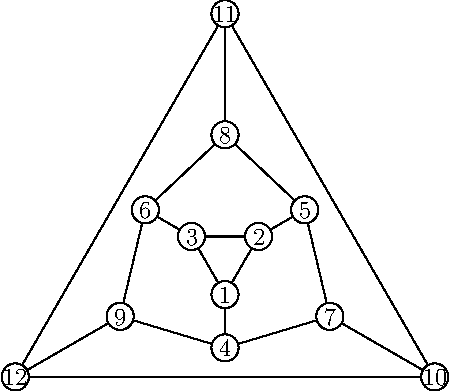
\includegraphics[scale=.8]{durer-graph-alt}
  \caption{The D\"urer graph, $D$.}
  \label{fig:durer-graph}
\end{figure}

\begin{solution}
  Rotating Figure~\ref{fig:durer-graph} by $120^\circ$ works.  In
  detail, the function maps $(1,2,3,\ 4,5,6,\ 7,8,9,\ 10,11,12)$ to
  $(2,3,1,\ 5,6,4,\ 8,9,7,\ 11,12,10)$ respectively.
\end{solution}

\ppart \label{InsideOutPart} Define a relation $R$ on $\vertices{G}$ by
declaring that $v\mrel{R}w$ precisely when there exists a graph
automorphism $f$ of $G$ with $f(v) = w$. In the special case of the
D{\"u}rer graph, prove that $1\mrel{R}10$.

\emph{Hint}: Try to map $1,2,3$ to $10,11,12$, respectively. Where must the other vertices go?
\begin{solution}
  It may be checked that the following function $g$ is an automorphism:
  \begin{align*}
    g(1) &\eqdef 10 & g(2) \eqdef 11 & g(3) \eqdef 12\\
    g(4) &\eqdef 7 & g(5) \eqdef 8 & g(6) \eqdef 9\\
    g(7) &\eqdef 5 & g(8) \eqdef 6 & g(9) \eqdef 4\\
    g(10) &\eqdef 2 & g(11) \eqdef 3 & g(12) \eqdef 1\\
  \end{align*}
\end{solution}

\ppart \label{NotInSameOrbitPart}
In the D\"urer graph, prove that $\QNOT(1\mrel{R}4)$.

\hint Length $3$ cycles.

\begin{solution}
  Let $f$ be any automorphism of $D$.  Because edges $\edge{1}{2}$,
  $\edge{2}{3}$, and $\edge{3}{1}$ exist in $D$, the edges
  $\edge{a}{b}$, $\edge{b}{c}$, and $\edge{c}{a}$ must also exist,
  where $a=f(1)$, $b=f(2)$, and $c=f(3)$.  In other words, $a,b,c$
  must form a length $3$ cycle in $D$.  But the only such cycles are
  $(1,2,3)$ and $(10,11,12)$, so $a=f(1)$ must be one of these six
  vertices.  In particular, $f(1)$ cannot be $4$.
\end{solution}

\ppart Prove carefully that for any simple graph $G$ (not necessarily
the D{\"u}rer graph), the relation $R$ defined above is an equivalence
relation.

\hint If $f$ and $g$ are graph automorphisms, prove that $g\circ f$
is, too.

\begin{solution}
  We must show $R$ is reflexive, symmetric, and transitive.

  \textbf{Reflexive}: the identity function $\ide: \vertices{G}\to \vertices{G}$ is a
  graph automorphism of $G$ and $\ide(v) = v$ for all vertices $v\in
  \vertices{G}$, so $v\mrel{R}v$ for all $v\in \vertices{G}$.

  \textbf{Transitive}: Assume $u\mrel{R}v$ and $v\mrel{R}w$; we must
  show $u\mrel{R}w$. We know there exist graph automorphisms $f$ and
  $g$ with $f(u) = v$ and $g(v) = w$; we'll show $g\circ f$ is also a
  graph automorphism.  Indeed, $g\circ f$ is a bijection of $\vertices{G}$
  with itself because $f$ and $g$ are each bijections. Next, for any
  nodes $p,q\in \vertices{G}$, we have
  \begin{equation*}
    \edge{p}{q} \in \edges{G} \QIFF \edge{f(p)}{f(q)} \in \edges{G} \QIFF
    \edge{g(f(p))}{g(f(q))} \in \edges{G},
  \end{equation*}
  using the facts that $f$ and $g$ are themselves graph automorphisms. This shows that $g\circ f$ is indeed a graph automorphism. Because $(g\circ f)(u) = w$, it follows that $u\, R\, w$.
  
\textbf{Symmetric}: If $v\, R\, w$, there must be a graph automorphism
$f$ of $G$ with $f(v) = w$. We'll show that $f^{-1}$ is also a graph
automorphism of $G$. First, $f^{-1}$ is a bijection of $\vertices{G}$
with itself because $f$ itself is. Next, for all vertices $p$ and $q$,
we have
\begin{align*}
  \lefteqn{\edge{f^{-1}(p)}{f^{-1}(q)}\in \edges{G}} \\
  & \QIFF \edge{f(f^{-1}(p))}{f(f^{-1}(q))} \in \edges{G} && \text{because $f$ is an automorphism} \\
  & \QIFF \edge{p}{q} \in \edges{G} && \text{because $f\circ f^{-1} = \ide$},
\end{align*}
so $f^{-1}$ is indeed a graph automorphism, and we have $f^{-1}(w) =
v$, so $w\mrel{R}v$.
\end{solution}

\ppart Because $R$ is an equivalence relation, it partitions the
vertices into equivalence classes.\footnote{Nodes in the same
  equivalence class can be thought of, informally, as having the
  ``same role'' in the graph, since you can move one to the other
  through an isomorphism.}  What are these equivalence classes for the
D{\"u}rer graph?  How do you know?

\emph{Hint}: There are only two classes.

\begin{solution}
We know that $1$ and $4$ are in different equivalence classes by
Part~\eqref{NotInSameOrbitPart}. On the other hand, the automorphism
in Part~\eqref{InsideOutPart} shows that $1,10,2,11,3,12$ must be in
the same equivalence class, as must $4,7,5,8,6,9$.  So the equivalence
classes are $\set{1,2,3,10,11,12}$ and $\set{4,5,6,7,8,9}$.
\end{solution}

\eparts


\end{problem}

%%%%%%%%%%%%%%%%%%%%%%%%%%%%%%%%%%%%%%%%%%%%%%%%%%%%%%%%%%%%%%%%%%%%%
% Problem ends here
%%%%%%%%%%%%%%%%%%%%%%%%%%%%%%%%%%%%%%%%%%%%%%%%%%%%%%%%%%%%%%%%%%%%%

\endinput
